% !TeX program = lualatex
% ================================================================
% Polish Parallel Text Version of CurrencyConversionGraphs
%
% Generated by the server using the following settings:
%
%   language            Polish (pol)
%   text direction      left to right
%   font                Noto Serif
%   fallback font       Noto Serif
%   built from          latex/worksheets/ratioAndProportion/currencyConversionGraphs.tex
%   vocabulary key      latex/worksheets/ratioAndProportion/currencyConversionGraphs/L2/pol/currencyConversionGraphs_polishKey.tex
%   tier 3 vocabulary   green   RGB 0 128 0
%   English text        black   RGB 0 0 0
%   Polish text         purple  RGB 112 48 160
%   layout macros       version 3
%
% Please don't edit any information in this comment block - the server
% compares it against the current settings and rebuilds this file when
% they differ, so changes here would be overwritten. However, feel free
% to make updates to the LaTeX below if you want to edit it.
% ================================================================

\documentclass[12pt,a4paper]{article}
% ================================================================
% Copied from the English sheet this was translated from, so that
% anything it sets up for itself still works here
% ================================================================
\usepackage[a4paper,top=12mm,bottom=14mm,left=15mm,right=15mm]{geometry}
\usepackage[T1]{fontenc}
\usepackage{amsmath}
\usepackage{amssymb}
\usepackage{enumitem}
\usepackage{multicol}
\usepackage{tikz}
\usepackage{pgfplots}
\pgfplotsset{compat=1.18}
\usepackage[most]{tcolorbox}
\usetikzlibrary{arrows.meta}

% ================================================================
% Currency conversion graphs.
%
% An extension sheet for ratio and proportion, designed to be worked
% through alone. It starts from the idea that a conversion graph
% with no fee is a straight line through the origin, and builds in
% four stages: matching lines to currencies by their steepness,
% measuring steepness as a gradient, adding a flat fee to give a
% y-intercept, and finding where two bureaux give the same amount by
% solving simultaneous equations. The sheet ends with open problems.
% Part 1 has no worked example: pupils find the link between the
% exchange rate and the steepness of a line for themselves in Q1,
% and then use it in Q2 and Q3.
% Pounds are on the x-axis throughout, apart from Q6, which turns the
% graph around on purpose. Answers are on the last page so that
% pupils can check each part before going on.
%
% The exchange rates are rounded versions of real rates, chosen so
% that every line passes through grid points and every step of the
% algebra comes out exactly.
%
% The sheet is written on, so every question is followed by a
% working area. The \newpage commands in the body are placed so
% that no question is split across the fold.
% ================================================================

\pagestyle{empty}
\linespread{1.15}\selectfont
\setlength{\parskip}{5pt}
\renewcommand{\arraystretch}{1.3}
\setlist[enumerate,1]{label=\textbf{Q\arabic*.}, leftmargin=*, itemsep=10pt, topsep=6pt, parsep=4pt}
\setlist[enumerate,2]{label=(\alph*), leftmargin=*, itemsep=8pt, topsep=5pt, parsep=3pt}
\setlength{\multicolsep}{4pt}
\setlength{\parindent}{0pt}

\newcommand{\ansline}[1][2.2cm]{\underline{\hspace{#1}}}
\newcommand{\zl}{z\l{}oty}

% A worked example: the method shown in full before it is practised.
% The boxes are drawn in pale tints, with a pale title bar, so that
% the printed sheet uses little toner.
\newtcolorbox{wex}[1]{colback=blue!2,colframe=blue!30,boxrule=0.6pt,
  colbacktitle=blue!8,coltitle=blue!50!black,
  left=6pt,right=6pt,top=4pt,bottom=5pt,
  title={\bfseries\small Worked example: #1},fonttitle=\small,
  toptitle=1pt,bottomtitle=1pt}

% The idea a section is built on, stated once and boxed.
\newtcolorbox{keyidea}{colback=orange!3,colframe=orange!35,boxrule=0.6pt,
  left=6pt,right=6pt,top=4pt,bottom=4pt}

% The section headings, kept tight so the parts do not eat the page.
\newcommand{\heading}[1]{%
  \vspace{2pt}
  {\color{blue!45!black}\rule{\linewidth}{1pt}}\\[1pt]
  {\large\bfseries #1}\\[-6pt]
  {\color{blue!45!black}\rule{\linewidth}{0.4pt}}
  \vspace{2pt}}
\newcommand{\parttitle}[2]{\heading{Part #1: #2}}

% ----------------------------------------------------------------
% Conversion graphs.
%
% Every graph uses the convgraph style: pounds along the x-axis,
% a light grid on the minor ticks and a darker one on the major
% ticks, and room outside the axes for the letter at the end of
% each line. The size and the scales are given at each graph.
% Graphs with a fee go below zero, so they use feegraph instead,
% which moves the x-axis up to y = 0.
\pgfplotsset{
  convgraph/.style={
    scale only axis,
    axis lines=left,
    axis line style={-},
    grid=both,
    major grid style={gray!55,line width=0.3pt},
    minor grid style={gray!20,line width=0.2pt},
    tick label style={font=\scriptsize},
    label style={font=\small},
    xlabel={Pounds (\pounds)},
    enlargelimits=false,
    clip=false,
    every axis plot/.append style={very thick,samples=2},
  },
  feegraph/.style={
    convgraph,
    axis x line=middle,
    axis y line=left,
    xlabel style={at={(rel axis cs:0.5,0)},anchor=north,yshift=-3pt},
  },
}
% The letter naming a line, written just past its end.
\newcommand{\linename}[1]{node[pos=1,right,font=\small\bfseries,text=black]{#1}}

\definecolor{lineA}{RGB}{0,90,170}
\definecolor{lineB}{RGB}{200,60,20}
\definecolor{lineC}{RGB}{20,130,60}

% Characters this language's font has not got are borrowed from another,
% rather than being silently dropped - see docs/translated-sheet-latex.md
\directlua{%
  if luaotfload and luaotfload.add_fallback then
    luaotfload.add_fallback("eallatinfallback",
      { "Noto Serif:mode=harf;" })
  else
    tex.error("this luaotfload is too old to register a fallback font")
  end
}
\usepackage[english]{babel}
\babelprovide[import]{polish}
\babelfont[polish]{rm}[Renderer=Harfbuzz, BoldFont={Noto Serif}, ItalicFont={Noto Serif}, BoldItalicFont={Noto Serif}, RawFeature={fallback=eallatinfallback}]{Noto Serif}
\babelfont[polish]{sf}[Renderer=Harfbuzz, BoldFont={Noto Serif}, ItalicFont={Noto Serif}, BoldItalicFont={Noto Serif}, RawFeature={fallback=eallatinfallback}]{Noto Serif}
\newcommand{\ealtext}[1]{\foreignlanguage{polish}{#1}}
\newcommand{\ealtextblock}[1]{{\raggedright\foreignlanguage{polish}{#1}\par}}
% ================================================================
% EAL layout helpers
% ================================================================
\usepackage{xcolor}

\definecolor{ealkeycolour}{RGB}{0,128,0}
\definecolor{ealenglish}{RGB}{0,0,0}
\definecolor{ealtwocolour}{RGB}{112,48,160}

\newsavebox{\ealboxen}
\newsavebox{\ealboxtr}
\newlength{\ealglosswd}
\newlength{\ealglossraise}
\setlength{\ealglossraise}{1.15em}

% a tier 3 word, in English and in translation alike
\newcommand{\ealkey}[1]{\textcolor{ealkeycolour}{#1}}
\newcommand{\ealkeytr}[1]{\textcolor{ealkeycolour}{\ealtext{#1}}}

% One translated word above one English word. Built from kernel
% primitives, never a tabular, which would break wherever the sheet
% loads array, booktabs or tabularx. The box is as wide as the wider of
% the two, so a long translation pushes its neighbours aside instead of
% overlapping them, and it claims its full height so a table row or a
% TikZ node makes room for it.
\newcommand{\ealgloss}[2]{%
  \sbox{\ealboxen}{\ealkey{#1}}%
  \sbox{\ealboxtr}{\small\textcolor{ealtwocolour}{\ealtext{#2}}}%
  \setlength{\ealglosswd}{\wd\ealboxen}%
  \ifdim\wd\ealboxtr>\ealglosswd\setlength{\ealglosswd}{\wd\ealboxtr}\fi
  \leavevmode
  \makebox[\ealglosswd][c]{%
    \makebox[0pt][c]{\usebox{\ealboxen}}%
    \makebox[0pt][c]{\raisebox{\ealglossraise}{\usebox{\ealboxtr}}}%
  }%
}

% opens up line spacing around a block of glosses, so the raised
% translations sit clear of the line above
\newenvironment{ealglossed}{\par\linespread{2.1}\selectfont\ignorespaces}{\par}

% a whole translated sentence above its English counterpart. block level,
% so it does not belong inside a tabular cell
\newcommand{\ealpara}[2]{%
  \par\addvspace{0.5\baselineskip}%
  {\color{ealtwocolour}\ealtextblock{#1}}%
  \penalty200
  {\color{ealenglish}#2\par}%
  \addvspace{0.5\baselineskip}%
}

\begin{document}

\begin{center}
  {\Large\bfseries \ealkey{Currency} \ealkey{Conversion Graphs}}\\[8pt]
\end{center}
\vspace{1pt}

\begin{keyidea}
\small
\ealpara
{A \textbf{\ealkeytr{kantor wymiany walut}} to miejsce, w którym wymienia się pieniądze z jednej \ealkeytr{waluty} na inną. \textbf{\ealkeytr{Kurs wymiany}} to ilość drugiej waluty, którą kupuje \pounds1. Gdy nie ma opłaty, ilość drugiej waluty jest \ealkeytr{wprost proporcjonalna} do liczby funtów, więc \ealkeytr{wykres przeliczeniowy} jest linią prostą przechodzącą przez \ealkeytr{początek układu współrzędnych}. Przejdź przez tę kartę, aby dowiedzieć się, jak stromość i położenie linii opisują wymianę.}
{A \textbf{\ealkey{bureau de change}} is a place where money is changed from one \ealkey{currency} into another. The \textbf{\ealkey{exchange rate}} is the amount of the other \ealkey{currency} that \pounds1 buys. When there is no fee, the amount of the other \ealkey{currency} is \ealkey{directly proportional} to the number of pounds, so the \ealkey{conversion graph} is a straight line through the \ealkey{origin}. Work through this sheet to find out how the steepness and the position of the line describe the exchange.}

\ealpara
{Kursy wymiany na tej karcie są zaokrąglone. Prawdziwe \ealkeytr{kursy wymiany} zmieniają się codziennie.}
{The \ealkey{exchange rates} in this sheet are rounded. Real \ealkey{exchange rates} change every day.}
\end{keyidea}

\ealpara{Która linia pokazuje którą \ealkeytr{walutę}?}{}
\parttitle{1}{Which line shows which \ealkey{currency}?}

\ealpara
{W każdym wykresie w tej części funty są na \ealkeytr{osi} x, a ilość innej \ealkeytr{waluty} jest na \ealkeytr{osi} y. Wykresy nie mówią, którą \ealkeytr{walutę} pokazuje każda linia: użyj \ealkeytr{kursów wymiany} z tabel, aby to ustalić.}
{In every graph in this part, pounds are on the \ealkey{x-axis} and the amount of another \ealkey{currency} is on the \ealkey{y-axis}. The graphs do not say which \ealkey{currency} each line shows: use the \ealkey{exchange rates} in the tables to work it out.}

\begin{enumerate}

\item \ealpara{Wykres pokazuje trzy \ealkeytr{wykresy przeliczeniowe}. Każda linia pokazuje jedną z \ealkeytr{walut} w tabeli.}{The graph shows three \ealkey{conversion graphs}. Each line shows one of the \ealkey{currencies} in the table.}
\vspace{2pt}

\begin{minipage}[t]{0.52\linewidth}
\centering
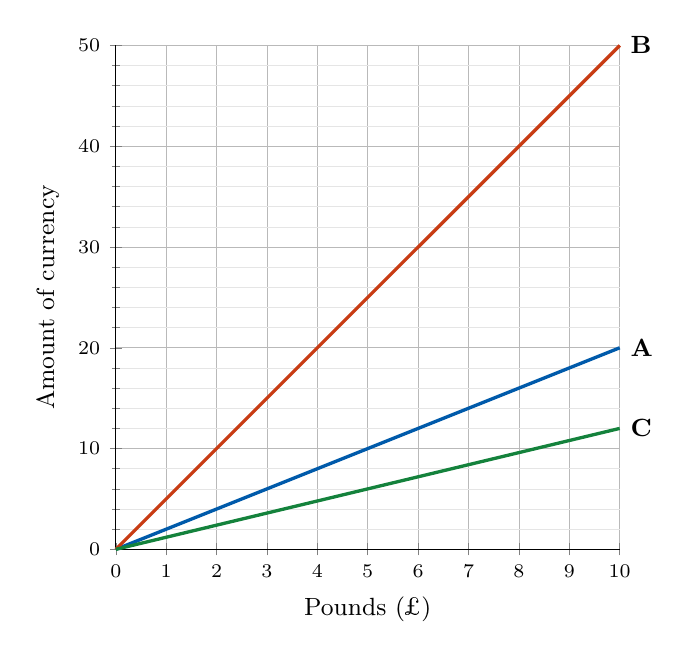
\begin{tikzpicture}[baseline=(current bounding box.north)]
\begin{axis}[convgraph,
    width=6.4cm,height=6.4cm,
    xmin=0,xmax=10,ymin=0,ymax=50,
    xtick distance=1,
    ytick distance=10,minor y tick num=4,
    ylabel={Amount of currency}]
  \addplot[lineA,domain=0:10] {2*x} \linename{A};
  \addplot[lineB,domain=0:10] {5*x} \linename{B};
  \addplot[lineC,domain=0:10] {1.2*x} \linename{C};
\end{axis}
\end{tikzpicture}
\end{minipage}%
\begin{minipage}[t]{0.48\linewidth}
\vspace{6pt}
\ealpara{\ealkeytr{Waluta} — ile kupuje \pounds1}{}
\begin{tabular}{|l|c|}
\hline
\textbf{\ealkey{Currency}} & \textbf{\pounds1 buys}\\
\hline
Euros (\texteuro) & $1.20$\\
\hline
Australian dollars & $2$\\
\hline
Polish \zl{} & $5$\\
\hline
\end{tabular}

\begin{enumerate}
  \item \ealpara{Która linia pokazuje dolary australijskie?}{Which line shows Australian dollars?}

        Line \ansline[2cm]
\end{enumerate}
\end{minipage}

\begin{enumerate}[start=2]
  \item \ealpara{Wyjaśnij, jak zdecydowałeś, która linia pokazuje dolary australijskie. Użyj w odpowiedzi każdego z tych słów.}{Explain how you decided which line shows Australian dollars. Use each of these words in your answer.}

        \begin{center}
        \fbox{\quad\textbf{steeper}\qquad\textbf{steepest}\qquad
        \textbf{less steep}\qquad\textbf{least steep}\quad}
        \end{center}

        \vspace{6em}
  \item \ealpara{Użyj wykresu, aby przeliczyć \pounds7 na dolary australijskie.}{Use the graph to convert \pounds7 into Australian dollars.}
        \hfill \ansline[2.5cm] Australian dollars
  \item \ealpara{Użyj wykresu, aby przeliczyć \texteuro6 na funty.}{Use the graph to convert \texteuro6 into pounds.}
        \hfill \pounds\ansline[2.5cm]
\end{enumerate}

\newpage

\item \ealpara{Tabela pokazuje, ile z czterech \ealkeytr{walut} kupuje \pounds1. Cztery \ealkeytr{wykresy przeliczeniowe} są narysowane na tych samych \ealkeytr{osiach}, z funtami na \ealkeytr{osi} x.}{The table shows how much of four \ealkey{currencies} \pounds1 buys. The four \ealkey{conversion graphs} are drawn on the same \ealkey{axes}, with pounds on the \ealkey{x-axis}.}
\vspace{2pt}

\begin{minipage}[t]{0.42\linewidth}
\vspace{4pt}
\ealpara{\ealkeytr{Waluta} — ile kupuje \pounds1}{}
\begin{tabular}{|l|c|}
\hline
\textbf{\ealkey{Currency}} & \textbf{\pounds1 buys}\\
\hline
Norwegian kroner & $13.50$\\
\hline
Indian rupees & $115$\\
\hline
Hong Kong dollars & $10.50$\\
\hline
Mexican pesos & $25$\\
\hline
\end{tabular}
\end{minipage}%
\begin{minipage}[t]{0.58\linewidth}
\centering
\begin{tikzpicture}[baseline=(current bounding box.north),font=\small]
  \draw[-{Stealth[length=2mm]}] (0,0) -- (8,0)
    node[anchor=north east,yshift=-2pt]{Pounds (\pounds)};
  \draw[-{Stealth[length=2mm]}] (0,0) -- (0,7)
    node[above]{Amount of currency};
  \node[below left] at (0,0) {$0$};
\end{tikzpicture}
\end{minipage}

\begin{enumerate}
  \item \ealpara{Naszkicuj cztery \ealkeytr{wykresy przeliczeniowe} na \ealkeytr{osiach}. \ealkeytr{Osie} nie muszą mieć skali, ale linie muszą być w prawidłowej kolejności stromości. Oznacz każdą linię jej \ealkeytr{walutą}.}{Sketch the four \ealkey{conversion graphs} on the \ealkey{axes}. The \ealkey{axes} do not need a scale, but the lines must be in the right order of steepness. Label each line with its \ealkey{currency}.}
  \item \ealpara{Wyjaśnij, dlaczego każda z czterech linii przechodzi przez \ealkeytr{początek układu współrzędnych}.}{Explain why every one of the four lines passes through the \ealkey{origin}.}

        \vspace{8em}
\end{enumerate}

\newpage

\item \ealpara{Wykres pokazuje trzy kolejne \ealkeytr{wykresy przeliczeniowe}, ale tym razem w tabeli jest pięć \ealkeytr{walut}. Dwie z \ealkeytr{walut} nie mają linii.}{The graph shows three more \ealkey{conversion graphs}, but this time there are five \ealkey{currencies} in the table. Two of the \ealkey{currencies} do not have a line.}
\vspace{2pt}

\begin{minipage}[t]{0.52\linewidth}
\centering
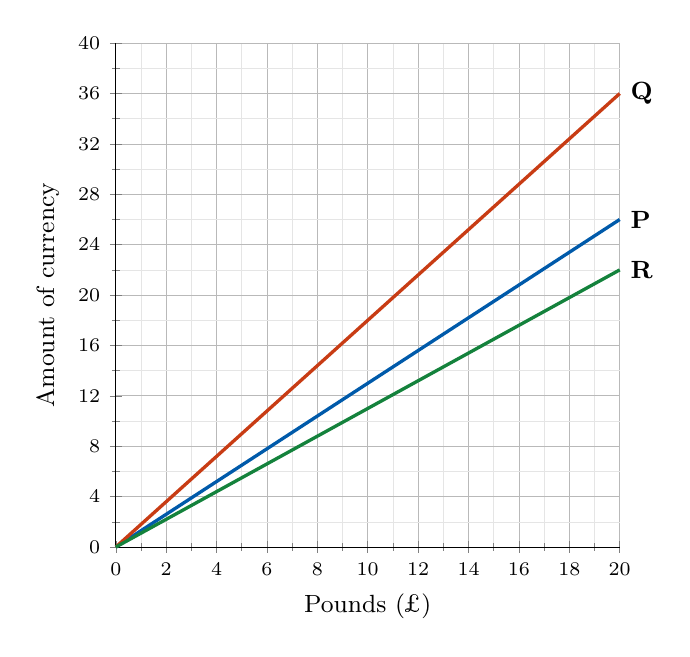
\begin{tikzpicture}[baseline=(current bounding box.north)]
\begin{axis}[convgraph,
    width=6.4cm,height=6.4cm,
    xmin=0,xmax=20,ymin=0,ymax=40,
    xtick distance=2,minor x tick num=1,
    ytick distance=4,minor y tick num=1,
    ylabel={Amount of currency}]
  \addplot[lineA,domain=0:20] {1.3*x} \linename{P};
  \addplot[lineB,domain=0:20] {1.8*x} \linename{Q};
  \addplot[lineC,domain=0:20] {1.1*x} \linename{R};
\end{axis}
\end{tikzpicture}
\end{minipage}%
\begin{minipage}[t]{0.48\linewidth}
\vspace{6pt}
\ealpara{\ealkeytr{Waluta} — ile kupuje \pounds1}{}
\begin{tabular}{|l|c|}
\hline
\textbf{\ealkey{Currency}} & \textbf{\pounds1 buys}\\
\hline
US dollars & $1.30$\\
\hline
Swiss francs & $1.10$\\
\hline
Canadian dollars & $1.80$\\
\hline
Singapore dollars & $1.70$\\
\hline
New Zealand dollars & $2.20$\\
\hline
\end{tabular}
\end{minipage}

\begin{enumerate}
  \item \ealpara{Zapisz \ealkeytr{walutę} pokazywaną przez każdą linię.}{Write down the \ealkey{currency} shown by each line.}

        Line P: \ansline[3.5cm] \quad Line Q: \ansline[3.5cm] \quad
        Line R: \ansline[3.5cm]

        \vspace{5em}
  \item \ealpara{Narysuj linie dla dolarów singapurskich i dolarów nowozelandzkich na wykresie. Oznacz każdą linię jej \ealkeytr{walutą}.}{Draw the lines for Singapore dollars and New Zealand dollars on the graph. Label each line with its \ealkey{currency}.}
  \item \ealpara{Sam mówi: „Linia Q jest najbardziej stromą linią, więc musi pokazywać dolary nowozelandzkie, ponieważ \pounds1 kupuje więcej dolarów nowozelandzkich niż jakakolwiek inna \ealkeytr{waluta} w tabeli.” Wyjaśnij, dlaczego Sam się myli.}{Sam says: ``Line Q is the steepest line, so it must show New Zealand dollars, because \pounds1 buys more New Zealand dollars than any other \ealkey{currency} in the table.'' Explain why Sam is wrong.}

        \vspace{7em}
\end{enumerate}

\end{enumerate}

\newpage

\ealpara{Mierzenie stromości za pomocą \ealkeytr{współczynnika kierunkowego}}{}
\parttitle{2}{Measuring steepness with the \ealkey{gradient}}

\ealpara
{Aby dokładnie porównać stromość, mierzymy ją liczbą zwaną \ealkeytr{współczynnikiem kierunkowym}. \ealkeytr{Współczynnik kierunkowy} prostej to odległość, o jaką linia wznosi się na każdy $1$ jednostkę w prawo:
\[
  \text{gradient}=\frac{\text{change in } y}{\text{change in } x}
\]
Na \ealkeytr{wykresie przeliczeniowym} $x$ oznacza liczbę funtów, a $y$ oznacza ilość innej \ealkeytr{waluty}. Przesunięcie $1$ jednostkę w prawo oznacza dodanie \pounds1, więc \ealkeytr{współczynnik kierunkowy} to \ealkeytr{kurs wymiany}. Prosta przechodząca przez \ealkeytr{początek układu współrzędnych} o \ealkeytr{współczynniku kierunkowym} $m$ ma \ealkeytr{równanie} $y=mx$ (pamiętaj $mx=m\times x$).}
{To compare steepness exactly, we measure it with a number called the \ealkey{gradient}. The \ealkey{gradient} of a straight line is how far the line rises for every $1$ unit it moves to the right:
\[
  \text{gradient}=\frac{\text{change in } y}{\text{change in } x}
\]
In a \ealkey{conversion graph}, $x$ stands for the number of pounds and $y$ stands for the amount of the other \ealkey{currency}. Moving $1$ unit to the right means adding \pounds1, so the \ealkey{gradient} is the \ealkey{exchange rate}. A straight line through the \ealkey{origin} with \ealkey{gradient} $m$ has the \ealkey{equation} $y=mx$ (remember $mx=m\times x$).}

\ealpara{Znajdź \ealkeytr{współczynnik kierunkowy} linii dirhama marokańskiego}{}
\begin{wex}{find the \ealkey{gradient} of the Moroccan dirham line}
\small
\begin{minipage}[t]{0.40\linewidth}
\centering
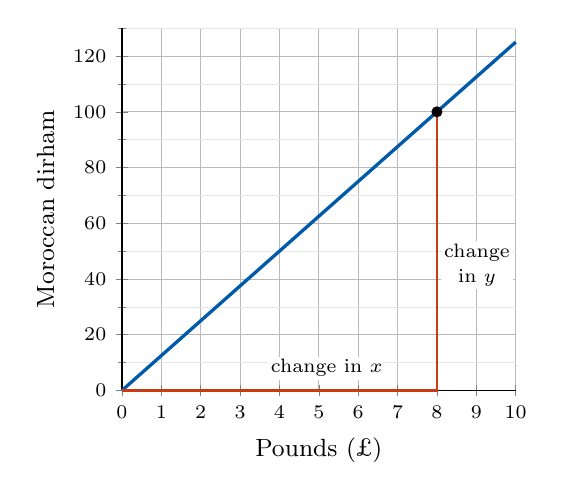
\begin{tikzpicture}[baseline=(current bounding box.north)]
\begin{axis}[convgraph,
    width=5cm,height=4.6cm,
    xmin=0,xmax=10,ymin=0,ymax=130,
    xtick distance=1,
    ytick distance=20,minor y tick num=1,
    ylabel={Moroccan dirham}]
  \addplot[lineA,domain=0:10] {12.5*x};
  \draw[lineB,thick] (axis cs:0,0) -- (axis cs:8,0) -- (axis cs:8,100);
  \fill (axis cs:8,100) circle (2pt);
  \node[font=\scriptsize,fill=white,inner sep=1pt] at (axis cs:5.2,8)
    {change in $x$};
  \node[font=\scriptsize,anchor=west,fill=white,inner sep=1pt] at
    (axis cs:8.1,45) {\shortstack{change\\in $y$}};
\end{axis}
\end{tikzpicture}
\end{minipage}%
\begin{minipage}[t]{0.60\linewidth}
\vspace{0pt}
\ealpara{Dwa punkty na linii; zmiana $x$; zmiana $y$; \ealkeytr{Współczynnik kierunkowy}; \ealkeytr{Równanie} linii; co oznacza \ealkeytr{współczynnik kierunkowy}}{}
\begin{tabular}{@{}l@{\hspace{0.8em}}l@{}}
\textbf{Two points on the line} & $(0,0)$ and $(8,100)$\\
\textbf{Change in $x$} & $8-0=8$\\
\textbf{Change in $y$} & $100-0=100$\\
\textbf{\ealkey{Gradient}} & $100\div8=12.5$\\
\textbf{\ealkey{Equation} of the line} & $y=12.5x$\\
\textbf{What the \ealkey{gradient} means} & \pounds1 buys $12.5$ dirham
\end{tabular}
\end{minipage}
\end{wex}

\begin{enumerate}[resume]

\item \ealpara{Wykres pokazuje \ealkeytr{wykres przeliczeniowy} dla randa południowoafrykańskiego. Uzupełnij luki, aby znaleźć jego \ealkeytr{współczynnik kierunkowy}.}{The graph shows the \ealkey{conversion graph} for South African rand. Fill in the gaps to find its \ealkey{gradient}.}
\vspace{2pt}

\begin{minipage}[t]{0.40\linewidth}
\centering
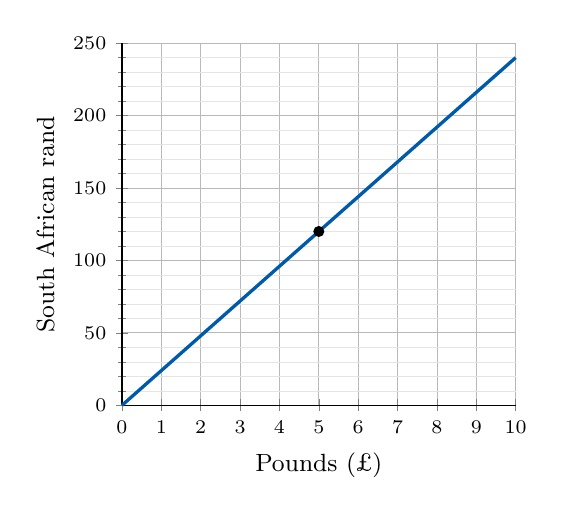
\begin{tikzpicture}[baseline=(current bounding box.north)]
\begin{axis}[convgraph,
    width=5cm,height=4.6cm,
    xmin=0,xmax=10,ymin=0,ymax=250,
    xtick distance=1,
    ytick distance=50,minor y tick num=4,
    ylabel={South African rand}]
  \addplot[lineA,domain=0:10] {24*x};
  \fill (axis cs:5,120) circle (2pt);
\end{axis}
\end{tikzpicture}
\end{minipage}%
\begin{minipage}[t]{0.60\linewidth}
\vspace{0pt}
\ealpara{Dwa punkty na linii; zmiana $x$; zmiana $y$; \ealkeytr{Współczynnik kierunkowy}; \ealkeytr{Równanie} linii; co oznacza \ealkeytr{współczynnik kierunkowy}}{}
\begin{tabular}{@{}l@{\hspace{0.8em}}l@{}}
\textbf{Two points on the line} & $(0,0)$ and $(5,\ansline[1.2cm])$\\[4pt]
\textbf{Change in $x$} & $5-0=\ansline[1.2cm]$\\[4pt]
\textbf{Change in $y$} & $\ansline[1.2cm]-0=\ansline[1.2cm]$\\[4pt]
\textbf{\ealkey{Gradient}} & $\ansline[1cm]\div\ansline[1cm]=\ansline[1cm]$\\[4pt]
\textbf{\ealkey{Equation} of the line} & $y=\ansline[1.2cm]\,x$\\[4pt]
\textbf{What the \ealkey{gradient} means} & \pounds1 buys \ansline[1.2cm] rand
\end{tabular}
\end{minipage}

\newpage

\item \ealpara{Wykres pokazuje dwa \ealkeytr{wykresy przeliczeniowe}. Jedna linia pokazuje jena japońskiego, a druga rupie pakistańskie. \pounds1 kupuje więcej rupii niż jenów.}{The graph shows two \ealkey{conversion graphs}. One line shows Japanese yen and the other shows Pakistani rupees. \pounds1 buys more rupees than yen.}
\vspace{2pt}

\begin{center}
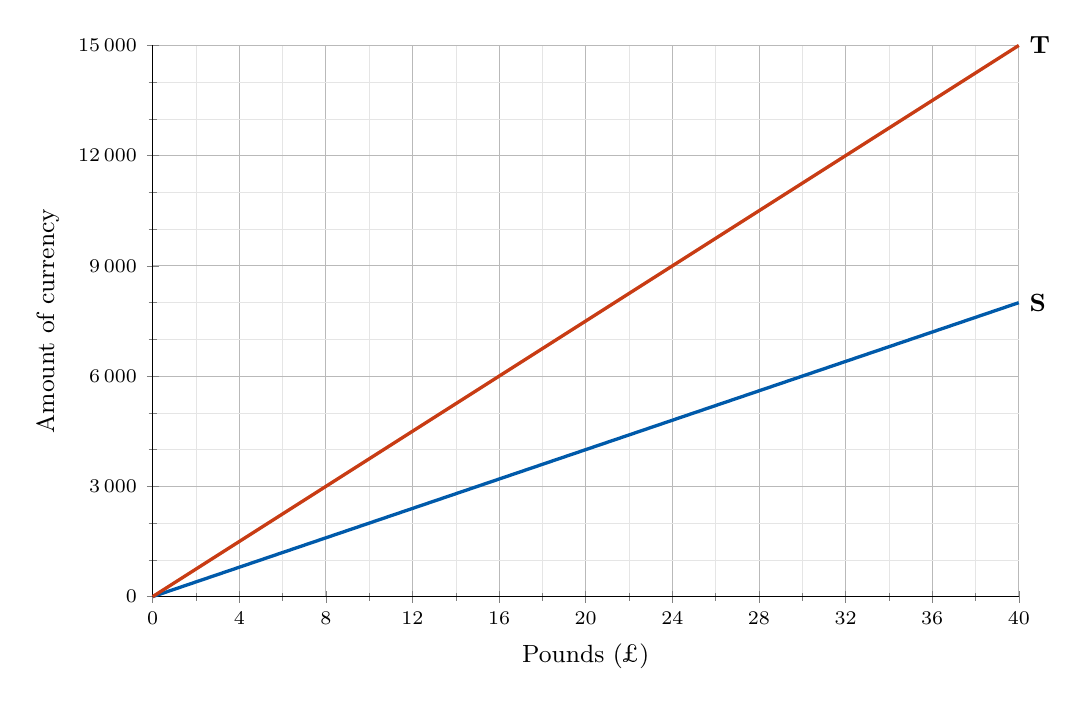
\begin{tikzpicture}
\begin{axis}[convgraph,
    width=11cm,height=7cm,
    xmin=0,xmax=40,ymin=0,ymax=15000,
    xtick distance=4,minor x tick num=1,
    ytick distance=3000,minor y tick num=2,
    scaled y ticks=false,
    yticklabel style={/pgf/number format/1000 sep={\,}},
    ylabel={Amount of currency}]
  \addplot[lineA,domain=0:40] {200*x} \linename{S};
  \addplot[lineB,domain=0:40] {375*x} \linename{T};
\end{axis}
\end{tikzpicture}
\end{center}

\begin{enumerate}
  \item \ealpara{Która linia pokazuje jena japońskiego? Podaj powód swojej odpowiedzi.}{Which line shows Japanese yen? Give a reason for your answer.}
        \hfill \ansline[3cm]

        \vspace{3em}
  \item \ealpara{Znajdź \ealkeytr{współczynnik kierunkowy} każdej linii i zapisz \ealkeytr{równanie} każdej linii. Rozpisz obliczenia tak jak w przykładzie.}{Find the \ealkey{gradient} of each line, and write down the \ealkey{equation} of each line. Set out your working like the worked example.}
        \vspace{4pt}

        \begin{minipage}[t]{0.48\linewidth}
        \textbf{Line S}\\[4pt]
        \ealpara{Dwa punkty na linii; zmiana $x$; zmiana $y$; \ealkeytr{Współczynnik kierunkowy}; \ealkeytr{Równanie}}{}
        \begin{tabular}{@{}l@{\hspace{0.6em}}l@{}}
        \textbf{Two points on the line} & \ansline[2.4cm]\\[5pt]
        \textbf{Change in $x$} & \ansline[2.4cm]\\[5pt]
        \textbf{Change in $y$} & \ansline[2.4cm]\\[5pt]
        \textbf{\ealkey{Gradient}} & \ansline[2.4cm]\\[5pt]
        \textbf{\ealkey{Equation}} & \ansline[2.4cm]
        \end{tabular}
        \end{minipage}\hfill
        \begin{minipage}[t]{0.48\linewidth}
        \textbf{Line T}\\[4pt]
        \ealpara{Dwa punkty na linii; zmiana $x$; zmiana $y$; \ealkeytr{Współczynnik kierunkowy}; \ealkeytr{Równanie}}{}
        \begin{tabular}{@{}l@{\hspace{0.6em}}l@{}}
        \textbf{Two points on the line} & \ansline[2.4cm]\\[5pt]
        \textbf{Change in $x$} & \ansline[2.4cm]\\[5pt]
        \textbf{Change in $y$} & \ansline[2.4cm]\\[5pt]
        \textbf{\ealkey{Gradient}} & \ansline[2.4cm]\\[5pt]
        \textbf{\ealkey{Equation}} & \ansline[2.4cm]
        \end{tabular}
        \end{minipage}
  \item \ealpara{Wykres kończy się na \pounds40. Użyj \ealkeytr{równania} linii S, aby przeliczyć \pounds250 na jeny.}{The graph stops at \pounds40. Use the \ealkey{equation} of line S to convert \pounds250 into yen.}

        \vspace{3.5em}
  \item \ealpara{Użyj \ealkeytr{równania} linii T, aby przeliczyć $30\,000$ rupii na funty.}{Use the \ealkey{equation} of line T to convert $30\,000$ rupees into pounds.}

        \vspace{4.5em}
\end{enumerate}

\newpage

\item \ealpara{Ola mieszka w Polsce i odwiedza Londyn. Rysuje \ealkeytr{wykres przeliczeniowy} w drugą stronę, z polskimi \zl{} na \ealkeytr{osi} x i funtami na \ealkeytr{osi} y. \ealkeytr{Kurs wymiany} wynosi \pounds1 $=5$ \zl{}.}{Ola lives in Poland and is visiting London. She draws a \ealkey{conversion graph} the other way round, with Polish \zl{} on the \ealkey{x-axis} and pounds on the \ealkey{y-axis}. The \ealkey{exchange rate} is \pounds1 $=5$ \zl{}.}
\vspace{2pt}

\begin{minipage}[t]{0.62\linewidth}
\centering
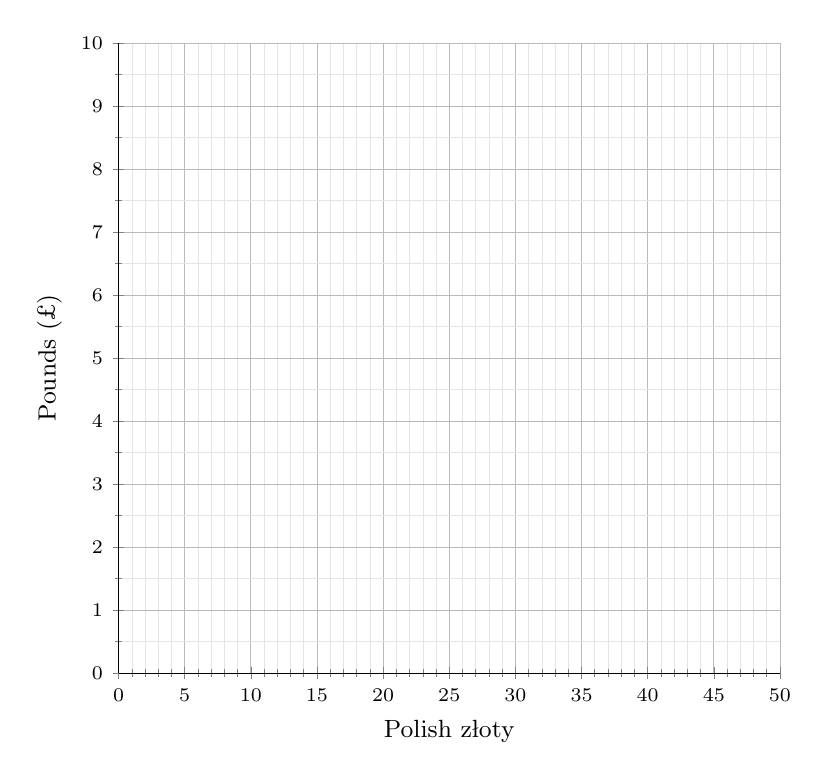
\begin{tikzpicture}[baseline=(current bounding box.north)]
\begin{axis}[convgraph,
    width=8.4cm,height=8cm,
    xmin=0,xmax=50,ymin=0,ymax=10,
    xtick distance=5,minor x tick num=4,
    ytick distance=1,minor y tick num=1,
    xlabel={Polish \zl{}},
    ylabel={Pounds (\pounds)}]
  \addplot[draw=none,domain=0:50] {0};
\end{axis}
\end{tikzpicture}
\end{minipage}%
\begin{minipage}[t]{0.38\linewidth}
\vspace{6pt}
\begin{tabular}{|l|c|c|c|c|}
\hline
\textbf{\zl{}} & $0$ & $10$ & $25$ & $50$\\
\hline
\textbf{\pounds} & $0$ & & & \\
\hline
\end{tabular}

\begin{enumerate}
  \item \ealpara{Uzupełnij tabelę.}{Complete the table.}
  \item \ealpara{Narysuj linię na siatce.}{Draw the line on the grid.}
\end{enumerate}
\end{minipage}

\begin{enumerate}[start=3]
  \item \ealpara{Znajdź \ealkeytr{współczynnik kierunkowy} linii Oli.}{Find the \ealkey{gradient} of Ola's line.} \hfill \ansline[3cm]

        \vspace{4em}
  \item \ealpara{Wyjaśnij, co \ealkeytr{współczynnik kierunkowy} linii Oli jej mówi.}{Explain what the \ealkey{gradient} of Ola's line tells her.}

        \vspace{6em}
\end{enumerate}

\end{enumerate}

\newpage

\ealpara{\ealkeytr{Stałe opłaty} i \ealkeytr{rzędna punktu przecięcia z osią Y}}{}
\parttitle{3}{\ealkey{Flat fees} and the \ealkey{y-intercept}}

\ealpara
{Niektóre \ealkeytr{kantory wymiany walut} pobierają \ealkeytr{stałą opłatę}: stałą kwotę, która jest odliczana od każdej wymiany, niezależnie od tego, ile pieniędzy się wymienia. Opłata jest odliczana najpierw, a pozostałe funty są przeliczane.}
{Some \ealkey{bureaux de change} charge a \ealkey{flat fee}: a fixed amount that is taken off every exchange, however much money is changed. The fee is taken off first, and the pounds that are left are converted.}

\ealpara
{Prosta o \ealkeytr{współczynniku kierunkowym} $m$, która przecina \ealkeytr{oś} y w $c$, ma \ealkeytr{równanie} $y=mx+c$. Liczba $c$ nazywa się \ealkeytr{rzędną punktu przecięcia z osią Y}. W kantorze ze \ealkeytr{stałą opłatą} \ealkeytr{współczynnik kierunkowy} nadal jest \ealkeytr{kursem wymiany}, a \ealkeytr{rzędna punktu przecięcia z osią Y} jest ujemna.}
{A straight line with \ealkey{gradient} $m$ that crosses the \ealkey{y-axis} at $c$ has the \ealkey{equation} $y=mx+c$. The number $c$ is called the \ealkey{y-intercept}. For a bureau with a \ealkey{flat fee}, the \ealkey{gradient} is still the \ealkey{exchange rate}, and the \ealkey{y-intercept} is negative.}

\ealpara{\ealkeytr{Stała opłata} \pounds5 i \texteuro1.20 za każde pozostałe \pounds1}{}
\begin{wex}{\pounds5 fee, and \texteuro1.20 for every \pounds1 left}
\small
\begin{minipage}[t]{0.40\linewidth}
\centering
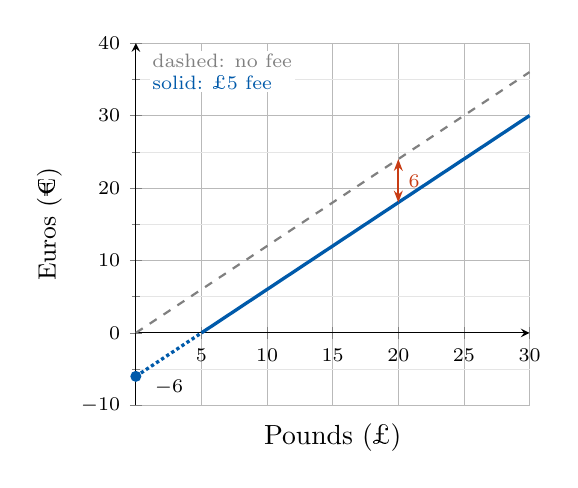
\begin{tikzpicture}[baseline=(current bounding box.north)]
\begin{axis}[feegraph,
    width=5cm,height=4.6cm,
    xmin=0,xmax=30,ymin=-10,ymax=40,
    xtick distance=5,
    ytick distance=10,minor y tick num=1,
    ylabel={Euros (\texteuro)}]
  \addplot[gray,dashed,thick,domain=0:30] {1.2*x};
  \addplot[lineA,densely dotted,domain=0:5] {1.2*x-6};
  \addplot[lineA,domain=5:30] {1.2*x-6};
  \node[font=\scriptsize,anchor=north west,align=left,fill=white,
    inner sep=1pt] at (axis cs:1,39)
    {\textcolor{gray}{dashed: no fee}\\\textcolor{lineA}{solid: \pounds5 fee}};
  \fill[lineA] (axis cs:0,-6) circle (2pt);
  \node[font=\scriptsize,anchor=west,fill=white,inner sep=1pt]
    at (axis cs:1.2,-7.5) {$-6$};
  \draw[{Stealth[length=1.5mm]}-{Stealth[length=1.5mm]},lineB,thick]
    (axis cs:20,24) -- (axis cs:20,18)
    node[midway,right,font=\scriptsize,text=lineB]{$6$};
\end{axis}
\end{tikzpicture}
\end{minipage}%
\begin{minipage}[t]{0.60\linewidth}
\vspace{0pt}
\ealpara
{Pozostałe funty do przeliczenia; otrzymane euro; \ealkeytr{Wymnóż nawiasy}; \ealkeytr{Współczynnik kierunkowy}; \ealkeytr{rzędna punktu przecięcia z osią Y}}{}
\begin{tabular}{@{}l@{\hspace{0.8em}}l@{}}
\textbf{Pounds converted} & $x-5$\\
\textbf{Euros received} & $y=1.2(x-5)$\\
\textbf{\ealkey{Expand} the brackets} & $y=1.2x-6$\\
\textbf{\ealkey{Gradient}} & $1.2$, the \ealkey{exchange rate}\\
\textbf{\ealkey{y-intercept}} & $-6$, the fee of \pounds5\\
 & is worth $1.2\times5=\text{\texteuro}6$
\end{tabular}

\smallskip
\ealpara
{Linia z opłatą jest \ealkeytr{równoległa} do linii bez opłaty, ponieważ \ealkeytr{kurs wymiany} jest taki sam. Jest o \texteuro6 niżej w każdym punkcie, ponieważ opłata jest warta \texteuro6. Kropkowana część linii jest tylko po to, aby pokazać, gdzie linia spotyka \ealkeytr{oś} y: wymiana mniej niż \pounds5 nie daje nic.}
{The fee line is \ealkey{parallel} to the no-fee line, because the \ealkey{exchange rate} is the same. It is \texteuro6 lower at every point, because the fee is worth \texteuro6. The dotted part of the line is only there to show where the line meets the \ealkey{y-axis}: exchanging less than \pounds5 gives nothing at all.}
\end{minipage}
\end{wex}

\begin{enumerate}[resume]

\item \ealpara{Bank pobiera \ealkeytr{stałą opłatę} \pounds10 i daje \$1.30 za każde pozostałe \pounds1. Uzupełnij luki, aby znaleźć \ealkeytr{równanie} jego \ealkeytr{wykresu przeliczeniowego}.}{A bank charges a \ealkey{flat fee} of \pounds10, and gives \$1.30 for every \pounds1 left. Fill in the gaps to find the \ealkey{equation} of its \ealkey{conversion graph}.}
\vspace{2pt}

\begin{minipage}[t]{0.40\linewidth}
\centering
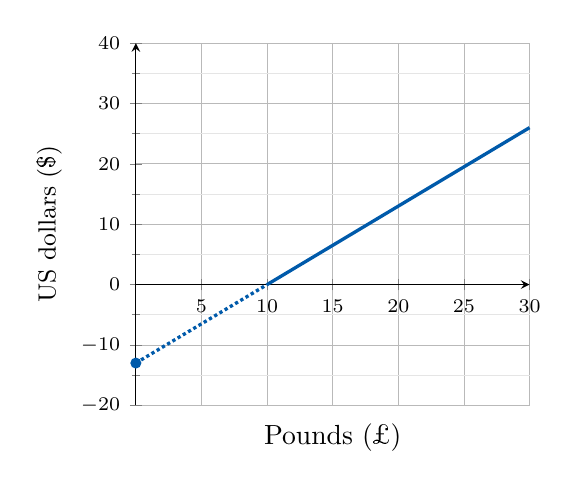
\begin{tikzpicture}[baseline=(current bounding box.north)]
\begin{axis}[feegraph,
    width=5cm,height=4.6cm,
    xmin=0,xmax=30,ymin=-20,ymax=40,
    xtick distance=5,
    ytick distance=10,minor y tick num=1,
    ylabel={US dollars (\$)}]
  \addplot[lineA,densely dotted,domain=0:10] {1.3*x-13};
  \addplot[lineA,domain=10:30] {1.3*x-13};
  \fill[lineA] (axis cs:0,-13) circle (2pt);
\end{axis}
\end{tikzpicture}
\end{minipage}%
\begin{minipage}[t]{0.60\linewidth}
\vspace{0pt}
\ealpara
{Pozostałe funty do przeliczenia; otrzymane dolary; \ealkeytr{Wymnóż nawiasy}; \ealkeytr{Współczynnik kierunkowy}; \ealkeytr{rzędna punktu przecięcia z osią Y}}{}
\begin{tabular}{@{}l@{\hspace{0.8em}}l@{}}
\textbf{Pounds converted} & $x-\ansline[1cm]$\\[4pt]
\textbf{Dollars received} & $y=\ansline[1cm](x-\ansline[1cm])$\\[4pt]
\textbf{\ealkey{Expand} the brackets} & $y=\ansline[1cm]\,x-\ansline[1cm]$\\[4pt]
\textbf{\ealkey{Gradient}} & \ansline[1cm], the \ealkey{exchange rate}\\[4pt]
\textbf{\ealkey{y-intercept}} & \ansline[1cm], the fee of \pounds\ansline[0.8cm]\\[4pt]
 & is worth $\ansline[0.8cm]\times\ansline[0.8cm]=\$\ansline[0.8cm]$
\end{tabular}
\end{minipage}

\begin{enumerate}
  \item \ealpara{Ile dolarów daje bank za \pounds100?}{How many dollars does the bank give for \pounds100?}
        \hfill \$\ansline[2.5cm]

        \vspace{3em}
  \item \ealpara{Jo chce otrzymać dokładnie \$130. Ile funtów musi wymienić?}{Jo wants to receive exactly \$130. How many pounds must she exchange?}
        \hfill \pounds\ansline[2.5cm]

        \vspace{5em}
\end{enumerate}

\newpage

\item \ealpara{Wykres pokazuje \ealkeytr{wykresy przeliczeniowe} dla trzech \ealkeytr{kantorów wymiany walut}. Jak w przykładzie, kropkowana część każdej linii pokazuje tylko, gdzie linia spotyka \ealkeytr{oś} y.}{The graph shows the \ealkey{conversion graphs} for three \ealkey{bureaux de change}. As in the worked example, the dotted part of each line only shows where the line meets the \ealkey{y-axis}.}
\vspace{2pt}

\begin{center}
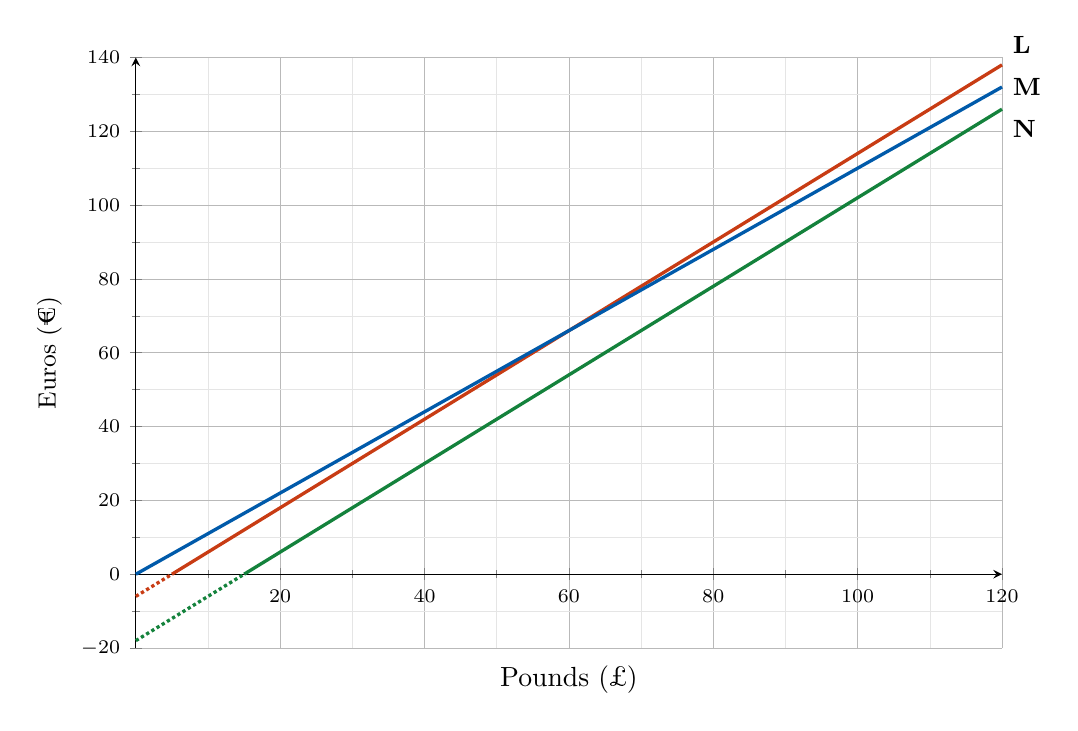
\begin{tikzpicture}
\begin{axis}[feegraph,
    width=11cm,height=7.5cm,
    xmin=0,xmax=120,ymin=-20,ymax=140,
    xtick distance=20,minor x tick num=1,
    ytick distance=20,minor y tick num=1,
    ylabel={Euros (\texteuro)}]
  \addplot[lineB,densely dotted,domain=0:5] {1.2*x-6};
  \addplot[lineB,domain=5:120] {1.2*x-6}
    node[pos=1,above right,font=\small\bfseries,text=black]{L};
  \addplot[lineA,domain=0:120] {1.1*x}
    node[pos=1,right,font=\small\bfseries,text=black]{M};
  \addplot[lineC,densely dotted,domain=0:15] {1.2*x-18};
  \addplot[lineC,domain=15:120] {1.2*x-18}
    node[pos=1,below right,font=\small\bfseries,text=black]{N};
\end{axis}
\end{tikzpicture}
\end{center}

\ealpara{Nazwa kantoru; \ealkeytr{stała opłata}; euro za każde pozostałe \pounds1; linia}{}
\begin{center}
\begin{tabular}{|l|c|c|c|}
\hline
\textbf{Bureau} & \textbf{\ealkey{Flat fee}} & \textbf{Euros for every \pounds1 left}
  & \textbf{Line}\\
\hline
Airport & none & $1.10$ & \\
\hline
High street & \pounds5 & $1.20$ & \\
\hline
Online & \pounds15 & $1.20$ & \\
\hline
\end{tabular}
\end{center}

\begin{enumerate}
  \item \ealpara{Uzupełnij tabelę, aby dopasować każdy kantor do jego linii.}{Complete the table to match each bureau to its line.}
  \item \ealpara{Dwie z linii są \ealkeytr{równoległe}. Wyjaśnij dlaczego.}{Two of the lines are \ealkey{parallel}. Explain why.}

        \vspace{3.5em}
  \item \ealpara{Zapisz \ealkeytr{równanie} każdej linii w postaci $y=mx+c$.}{Write down the \ealkey{equation} of each line in the form $y=mx+c$.}

        Line L: \ansline[3cm] \quad Line M: \ansline[3cm] \quad
        Line N: \ansline[3cm]
  \item \ealpara{Linie L i M przecinają się. Użyj wykresu, aby znaleźć liczbę funtów, przy której się przecinają, i wyjaśnij, co punkt przecięcia mówi ci o kantorze lotniskowym i kantorze przy głównej ulicy.}{Lines L and M cross. Use the graph to find the number of pounds where they cross, and explain what the crossing point tells you about the airport and the high street bureaux.}

        \vspace{6em}
\end{enumerate}

\newpage

\item \ealpara{\ealkeytr{Wykres przeliczeniowy} kantoru dla dolarów kanadyjskich ma \ealkeytr{równanie}
\[
  y=1.8x-9
\]
gdzie $x$ to liczba wymienianych funtów, a $y$ to liczba otrzymanych dolarów kanadyjskich.}{\ealkey{A conversion graph} for a bureau for Canadian dollars has the \ealkey{equation}
\[
  y=1.8x-9
\]
where $x$ is the number of pounds exchanged and $y$ is the number of Canadian dollars received.}
\begin{enumerate}
  \item \ealpara{Jaki jest \ealkeytr{kurs wymiany} w tym kantorze?}{What is the \ealkey{exchange rate} at this bureau?} \hfill \ansline[3cm]

        \vspace{2em}
  \item \ealpara{Jaką \ealkeytr{stałą opłatę} pobiera kantor, w funtach? Pokaż, jak to obliczyłeś.}{What \ealkey{flat fee} does the bureau charge, in pounds? Show how you worked it out.}

        \vspace{6em}
  \item \ealpara{Wyjaśnij, dlaczego ten kantor nie daje w ogóle dolarów kanadyjskich osobie, która wymienia \pounds5.}{Explain why this bureau gives no Canadian dollars at all to someone who exchanges \pounds5.}

        \vspace{6em}
  \item \ealpara{Drugi kantor ma taki sam \ealkeytr{kurs wymiany}, ale pobiera \ealkeytr{stałą opłatę} \pounds10. Zapisz \ealkeytr{równanie} jego \ealkeytr{wykresu przeliczeniowego} i opisz, jak jego linia wypada w porównaniu z linią $y=1.8x-9$.}{A second bureau has the same \ealkey{exchange rate}, but charges a \ealkey{flat fee} of \pounds10. Write down the \ealkey{equation} of its \ealkey{conversion graph}, and describe how its line compares with the line $y=1.8x-9$.}

        \vspace{8em}
\end{enumerate}

\end{enumerate}

\newpage

\ealpara{Kiedy dwa kantory dają tę samą kwotę?}{}
\parttitle{4}{When do two bureaux give the same amount?}

\ealpara
{Gdy dwa \ealkeytr{wykresy przeliczeniowe} się przecinają, dwa kantory dają tę samą ilość \ealkeytr{waluty} za tę samą liczbę funtów. Aby dokładnie znaleźć punkt przecięcia, przyrównujemy do siebie dwa \ealkeytr{wyrażenia} na $y$ i \ealkeytr{rozwiązujemy} \ealkeytr{równanie}. Znalezienie wartości $x$ i $y$, które sprawiają, że dwa równania są prawdziwe jednocześnie, nazywa się \ealkeytr{rozwiązywaniem układów równań}.}
{Where two \ealkey{conversion graphs} cross, the two bureaux give the same amount of \ealkey{currency} for the same number of pounds. To find the crossing point exactly, we set the two \ealkey{expressions} for $y$ equal to each other and \ealkey{solve} the \ealkey{equation}. Finding the values of $x$ and $y$ that make two equations true at the same time is called \ealkey{solving} \ealkey{simultaneous equations}.}

\ealpara{Kantor lotniskowy i kantor przy głównej ulicy z Q8}{}
\begin{wex}{the airport and the high street bureau from Q8}
\small
\ealpara
{\textbf{Lotnisko:} bez opłaty, \texteuro1.10 za każde \pounds1, więc $y=1.1x$.\\
\textbf{Główna ulica:} opłata \pounds5, \texteuro1.20 za każde pozostałe \pounds1, więc
$y=1.2(x-5)=1.2x-6$.}
{\textbf{Airport:} no fee, \texteuro1.10 for every \pounds1, so $y=1.1x$.\\
\textbf{High street:} \pounds5 fee, \texteuro1.20 for every \pounds1 left, so
$y=1.2(x-5)=1.2x-6$.}

\ealpara{Funty, $x$; Lotnisko, $y$; Główna ulica, $y$}{}
\begin{center}
\begin{tabular}{|l|c|c|c|c|}
\hline
\textbf{Pounds, $x$} & $0$ & $40$ & $80$ & $120$\\
\hline
\textbf{Airport, $y$} & $0$ & $44$ & $88$ & $132$\\
\hline
\textbf{High street, $y$} & $-6$ & $42$ & $90$ & $138$\\
\hline
\end{tabular}
\end{center}

\begin{minipage}[t]{0.44\linewidth}
\centering
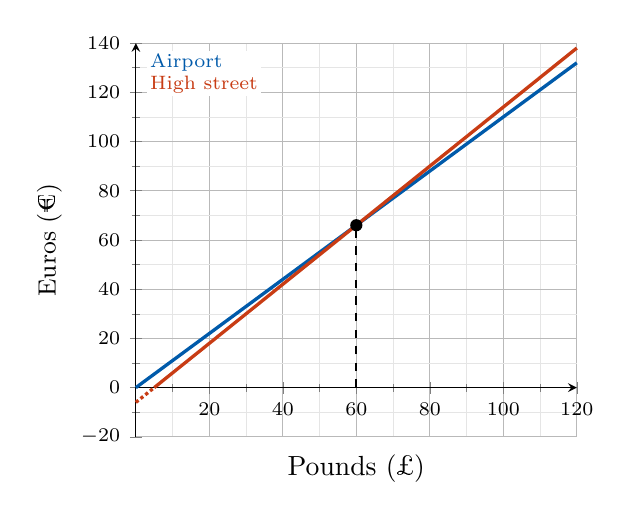
\begin{tikzpicture}[baseline=(current bounding box.north)]
\begin{axis}[feegraph,
    width=5.6cm,height=5cm,
    xmin=0,xmax=120,ymin=-20,ymax=140,
    xtick distance=20,minor x tick num=1,
    ytick distance=20,minor y tick num=1,
    ylabel={Euros (\texteuro)}]
  \addplot[lineA,domain=0:120] {1.1*x};
  \addplot[lineB,densely dotted,domain=0:5] {1.2*x-6};
  \addplot[lineB,domain=5:120] {1.2*x-6};
  \draw[dashed,thick] (axis cs:60,0) -- (axis cs:60,66);
  \fill (axis cs:60,66) circle (2.2pt);
  \node[font=\scriptsize,anchor=north west,align=left,fill=white,
    inner sep=1pt] at (axis cs:3,137)
    {\textcolor{lineA}{Airport}\\\textcolor{lineB}{High street}};
\end{axis}
\end{tikzpicture}
\end{minipage}%
\begin{minipage}[t]{0.56\linewidth}
\vspace{0pt}
\ealpara
{Linia głównej ulicy jest poniżej linii lotniska przy \pounds40 i powyżej niej przy \pounds80, więc linie przecinają się między \pounds40 a \pounds80.}
{The high street line is below the airport line at \pounds40 and above it at \pounds80, so the lines cross between \pounds40 and \pounds80.}

\ealpara
{Ta sama kwota, gdy; odejmij $1.1x$ od obu stron; dodaj $6$ do obu stron; pomnóż obie strony przez $10$; otrzymane euro}{}
\begin{tabular}{@{}l@{\hspace{0.8em}}l@{}}
\textbf{Same amount when} & $1.1x=1.2x-6$\\
\textbf{Subtract $1.1x$ from both sides} & $0=0.1x-6$\\
\textbf{Add $6$ to both sides} & $6=0.1x$\\
\textbf{Multiply both sides by $10$} & $60=x$\\
\textbf{Euros received} & $y=1.1\times60=66$
\end{tabular}
\end{minipage}

\ealpara
{Obydwa kantory dają \texteuro66 za \pounds60. Za mniej niż \pounds60 lotnisko daje więcej euro, ponieważ jego linia jest wyżej. Za więcej niż \pounds60 kantor przy głównej ulicy daje więcej euro, ponieważ jego linia jest bardziej stroma i jest teraz wyższą linią.}
{Both bureaux give \texteuro66 for \pounds60. For less than \pounds60 the airport gives more euros, because its line is higher. For more than \pounds60 the high street bureau gives more euros, because its line is steeper and is now the higher line.}
\end{wex}

\begin{enumerate}[resume]

\item \ealpara{Użyj przykładu, aby odpowiedzieć na te pytania.}{Use the worked example to answer these.}
\begin{enumerate}
  \item \ealpara{Ile euro daje każdy kantor za \pounds30? Który kantor daje więcej?}{How many euros does each bureau give for \pounds30? Which bureau gives more?}

        \vspace{4em}
  \item \ealpara{Ile euro daje każdy kantor za \pounds200? Który kantor daje więcej i o ile więcej?}{How many euros does each bureau give for \pounds200? Which bureau gives more, and how many more?}

        \vspace{4em}
  \item \ealpara{Gdy linie się przetną, różnica między dwoma kantorami rośnie wraz ze wzrostem liczby funtów. Użyj \ealkeytr{współczynników kierunkowych} tych dwóch linii, aby wyjaśnić dlaczego.}{Once the lines have crossed, the difference between the two bureaux gets bigger as the number of pounds goes up. Use the \ealkey{gradients} of the two lines to explain why.}

        \vspace{5em}
\end{enumerate}

\newpage

\item \ealpara{Kantor lotniskowy i kantor w mieście wymieniają funty na polskie \zl{}. Uzupełnij luki w \ealkeytr{równaniach}, tabeli i obliczeniach, tak jak w przykładzie.}{An airport bureau and a bureau in town both change pounds into Polish \zl{}. Fill in the gaps in the \ealkey{equations}, the table and the working, as in the worked example.}

\medskip
\ealpara
{\textbf{Lotnisko:} bez opłaty, $4.50$ \zl{} za każde \pounds1, więc
$y=\ansline[1.2cm]\,x$.\\[4pt]
\textbf{Miasto:} opłata \pounds3, $5$ \zl{} za każde pozostałe \pounds1, więc
$y=5(x-\ansline[1cm])=\ansline[1cm]\,x-\ansline[1cm]$.}
{\textbf{Airport:} no fee, $4.50$ \zl{} for every \pounds1, so
$y=\ansline[1.2cm]\,x$.\\[4pt]
\textbf{Town:} \pounds3 fee, $5$ \zl{} for every \pounds1 left, so
$y=5(x-\ansline[1cm])=\ansline[1cm]\,x-\ansline[1cm]$.}

\ealpara{Funty, $x$; Lotnisko, $y$; Miasto, $y$}{}
\begin{center}
\begin{tabular}{|l|c|c|c|c|}
\hline
\textbf{Pounds, $x$} & $0$ & $20$ & $40$ & $60$\\
\hline
\textbf{Airport, $y$} & $0$ & \hspace{1.2cm} & \hspace{1.2cm} & \hspace{1.2cm}\\
\hline
\textbf{Town, $y$} & & & & \\
\hline
\end{tabular}
\end{center}

\begin{minipage}[t]{0.42\linewidth}
\centering
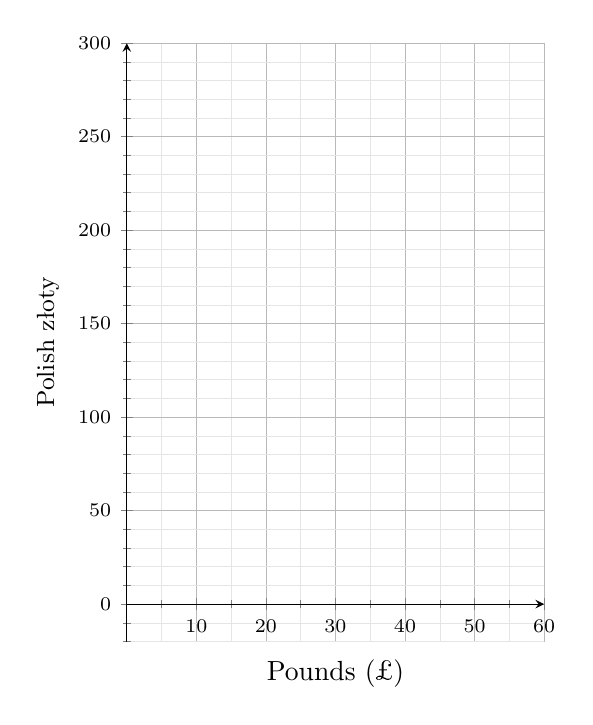
\begin{tikzpicture}[baseline=(current bounding box.north)]
\begin{axis}[feegraph,
    width=5.3cm,height=7.6cm,
    xmin=0,xmax=60,ymin=-20,ymax=300,
    xtick distance=10,minor x tick num=1,
    ytick distance=50,minor y tick num=4,
    ylabel={Polish \zl{}}]
  \addplot[draw=none,domain=0:60] {0};
\end{axis}
\end{tikzpicture}
\end{minipage}%
\begin{minipage}[t]{0.58\linewidth}
\vspace{0pt}
\ealpara
{Linia miasta jest \ansline[1.4cm] linią lotniska przy \pounds20 i \ansline[1.4cm] nią przy \pounds40, więc linie przecinają się między \pounds20 a \pounds40.}
{The town line is \ansline[1.4cm] the airport line at \pounds20 and \ansline[1.4cm] it at \pounds40, so the lines cross between \pounds20 and \pounds40.}

\ealpara
{Ta sama kwota, gdy; odejmij $4.5x$ od obu stron; dodaj \ansline[0.8cm] do obu stron; pomnóż obie strony przez \ansline[0.8cm]; otrzymane złote}{}
\begin{tabular}{@{}l@{\hspace{0.5em}}l@{}}
\textbf{Same amount when} & $\ansline[1.2cm]=\ansline[1.4cm]$\\[5pt]
\textbf{Subtract $4.5x$ from both sides} & $0=\ansline[0.8cm]\,x-\ansline[0.8cm]$\\[5pt]
\textbf{Add \ansline[0.8cm] to both sides} & $\ansline[0.8cm]=0.5x$\\[5pt]
\textbf{Multiply both sides by \ansline[0.8cm]} & $\ansline[0.8cm]=x$\\[5pt]
\textbf{Z\l{}oty received} & $y=\ansline[1.6cm]$
\end{tabular}
\end{minipage}

\begin{enumerate}
  \item \ealpara{Narysuj obie linie na siatce i zaznacz punkt, w którym się przecinają.}{Draw both lines on the grid, and mark the point where they cross.}
  \item \ealpara{Który kantor daje więcej \zl{} za \pounds20?}{Which bureau gives more \zl{} for \pounds20?} \hfill \ansline[3cm]
  \item \ealpara{Który kantor daje więcej \zl{} za \pounds50?}{Which bureau gives more \zl{} for \pounds50?} \hfill \ansline[3cm]
\end{enumerate}

\newpage

\item \ealpara{Kantor lotniskowy daje \$1.15 za każde \pounds1 i nie pobiera opłaty. Kantor internetowy pobiera \ealkeytr{stałą opłatę} \pounds8 i daje \$1.25 za każde pozostałe \pounds1.}{The airport bureau gives \$1.15 for every \pounds1 and charges no fee. An online bureau charges a \ealkey{flat fee} of \pounds8 and gives \$1.25 for every \pounds1 left.}
\begin{enumerate}
  \item \ealpara{Zapisz \ealkeytr{równanie} każdego \ealkeytr{wykresu przeliczeniowego}.}{Write down the \ealkey{equation} of each \ealkey{conversion graph}.}

        \vspace{4em}
  \item \ealpara{Znajdź liczbę funtów, dla której oba kantory dają tę samą liczbę dolarów, i ile to dolarów.}{Find the number of pounds for which both bureaux give the same number of dollars, and how many dollars that is.}

        \vspace{9em}
  \item \ealpara{Mia wymienia \pounds400 na wakacje w Nowym Jorku. Który kantor powinna wybrać i o ile więcej dolarów otrzyma?}{Mia is exchanging \pounds400 for a holiday in New York. Which bureau should she use, and how many more dollars will she get?}

        \vspace{6em}
\end{enumerate}

\item \ealpara{Dwa kantory pobierają \ealkeytr{stałą opłatę}. Kantor E pobiera \pounds2 i daje $190$ jenów japońskich za każde pozostałe \pounds1. Kantor F pobiera \pounds5 i daje $200$ jenów za każde pozostałe \pounds1.}{Two bureaux both charge a \ealkey{flat fee}. Bureau E charges \pounds2 and gives $190$ Japanese yen for every \pounds1 left. Bureau F charges \pounds5 and gives $200$ yen for every \pounds1 left.}
\begin{enumerate}
  \item \ealpara{Pokaż, że \ealkeytr{równanie} dla kantoru E to $y=190x-380$, i zapisz \ealkeytr{równanie} dla kantoru F.}{Show that the \ealkey{equation} for Bureau E is $y=190x-380$, and write down the \ealkey{equation} for Bureau F.}

        \vspace{4em}
  \item \ealpara{Znajdź liczbę funtów, dla której oba kantory dają tę samą liczbę jenów.}{Find the number of pounds for which both bureaux give the same number of yen.}

        \vspace{7em}
  \item \ealpara{Kenji ma \pounds500 do wymiany. Który kantor powinien wybrać i o ile więcej jenów otrzyma?}{Kenji has \pounds500 to exchange. Which bureau should he use, and how many more yen will he get?}

        \vspace{5em}
\end{enumerate}

\end{enumerate}

\newpage

\ealpara{Wyzwania}{}
\parttitle{5}{Challenges}

\begin{enumerate}[resume]

\item \ealpara{Dwa kantory pobierają \ealkeytr{stałą opłatę} \pounds5. Kantor G daje \texteuro1.10 za każde pozostałe \pounds1, a kantor H daje \texteuro1.20 za każde pozostałe \pounds1.}{Two bureaux both charge a \ealkey{flat fee} of \pounds5. Bureau G gives \texteuro1.10 for every \pounds1 left, and Bureau H gives \texteuro1.20 for every \pounds1 left.}
\begin{enumerate}
  \item \ealpara{Zapisz \ealkeytr{równanie} każdego \ealkeytr{wykresu przeliczeniowego} i \ealkeytr{rzędną punktu przecięcia z osią Y} każdej linii.}{Write down the \ealkey{equation} of each \ealkey{conversion graph}, and the \ealkey{y-intercept} of each line.}

        \vspace{4.5em}
  \item \ealpara{Pokaż, że obie linie przecinają \ealkeytr{oś} x w $x=5$, i wyjaśnij, co oznacza ten punkt.}{Show that both lines cross the \ealkey{x-axis} at $x=5$, and explain what this point means.}

        \vspace{6em}
  \item \ealpara{Tom mówi: „Jeśli dwa kantory pobierają tę samą \ealkeytr{stałą opłatę}, kantor z lepszym \ealkeytr{kursem wymiany} zawsze daje więcej euro.” Użyj swoich odpowiedzi do podpunktów (a) i (b), aby zdecydować, czy Tom ma rację.}{Tom says: ``If two bureaux charge the same \ealkey{flat fee}, the bureau with the better \ealkey{exchange rate} always gives more euros.'' Use your answers to parts (a) and (b) to decide whether Tom is right.}

        \vspace{8em}
\end{enumerate}

\item \ealpara{Kantor lotniskowy daje \texteuro1.10 za każde \pounds1 i nie pobiera opłaty. Zaprojektuj ofertę dla nowego kantoru, ze \ealkeytr{stałą opłatą} i lepszym \ealkeytr{kursem wymiany}, tak aby nowy kantor i lotnisko dawały tę samą liczbę euro, gdy wymienia się dokładnie \pounds300. Pokaż, że twoja oferta działa, i wyjaśnij, kto powinien użyć nowego kantoru zamiast lotniska.}{The airport bureau gives \texteuro1.10 for every \pounds1 and charges no fee. Design a deal for a new bureau, with a \ealkey{flat fee} and a better \ealkey{exchange rate}, so that the new bureau and the airport give the same number of euros when exactly \pounds300 is exchanged. Show that your deal works, and explain who should use the new bureau rather than the airport.}

\vspace{12em}

\newpage

\item \ealpara{Niektóre kantory pobierają \ealkeytr{prowizję} zamiast \ealkeytr{stałej opłaty}. \ealkeytr{Prowizja} to \ealkeytr{procent} wymienianych funtów. Kantor K pobiera $2\%$ \ealkeytr{prowizji} i daje \texteuro1.25 za każde pozostałe \pounds1.}{Some bureaux charge a \ealkey{commission} instead of a \ealkey{flat fee}. A \ealkey{commission} is a \ealkey{percentage} of the pounds exchanged. Bureau K takes $2\%$ \ealkey{commission}, and gives \texteuro1.25 for every \pounds1 left.}
\begin{enumerate}
  \item \ealpara{Pokaż, że wymiana \pounds100 w kantorze K daje \texteuro122.50.}{Show that exchanging \pounds100 at Bureau K gives \texteuro122.50.}

        \vspace{5em}
  \item \ealpara{Aisha mówi: „\ealkeytr{Prowizja} to rodzaj opłaty, więc linia kantoru K przecina \ealkeytr{oś} y poniżej zera, tak jak linia kantoru przy głównej ulicy.” Wyjaśnij, czy Aisha ma rację, i znajdź \ealkeytr{współczynnik kierunkowy} linii kantoru K.}{Aisha says: ``A \ealkey{commission} is a kind of fee, so the line for Bureau K crosses the \ealkey{y-axis} below zero, like the line for the high street bureau.'' Explain whether Aisha is right, and find the \ealkey{gradient} of the line for Bureau K.}

        \vspace{9em}
  \item \ealpara{Czy kantor K jest lepszy, czy gorszy od kantoru przy głównej ulicy (opłata \pounds5, \texteuro1.20 za każde pozostałe \pounds1)? Czy twoja odpowiedź zależy od tego, ile funtów się wymienia? Wyjaśnij, używając \ealkeytr{równań} tych dwóch linii.}{Is Bureau K better or worse than the high street bureau (\pounds5 fee, \texteuro1.20 for every \pounds1 left)? Does your answer depend on how many pounds are exchanged? Explain using the \ealkey{equations} of the two lines.}

        \vspace{12em}
\end{enumerate}

\end{enumerate}

\newpage

\ealpara{Odpowiedzi}{}
\heading{Answers}

{\small
\begin{multicols}{2}
\raggedcolumns
\setlength{\parskip}{4pt}

\ealpara
{\textbf{Q1.} (a) Linia A. \quad
(b) Na przykład: \pounds1 kupuje więcej \zl{} niż którakolwiek z pozostałych \ealkeytr{walut}, więc każdy \pounds1 dodaje najwięcej do linii \zl{}, a linia \zl{} jest najbardziej stromą linią, B. \pounds1 kupuje najmniej euro, więc linia euro jest najmniej stromą linią, C. \pounds1 kupuje $2$ dolary australijskie, co jest więcej niż \texteuro1.20 i mniej niż $5$ \zl{}, więc linia dolara australijskiego jest bardziej stroma niż linia euro i mniej stroma niż linia \zl{}. To jest linia A. \quad
(c) $14$ dolarów australijskich. \quad
(d) \pounds5, odczytane z linii C.}
{\textbf{Q1.} (a) Line A. \quad
(b) For example: \pounds1 buys more \zl{} than either of the other \ealkey{currencies}, so each \pounds1 adds the most to the \zl{} line, and the \zl{} line is the steepest line, B. \pounds1 buys the fewest euros, so the euro line is the least steep line, C. \pounds1 buys $2$ Australian dollars, which is more than \texteuro1.20 and fewer than $5$ \zl{}, so the Australian dollar line is steeper than the euro line and less steep than the \zl{} line. That is line A. \quad
(c) $14$ Australian dollars. \quad
(d) \pounds5, reading from line C.}

\ealpara
{\textbf{Q2.} (a) Od najbardziej stromej linii do najmniej stromej: rupie indyjskie ($115$), peso meksykańskie ($25$), korony norweskie ($13.50$), dolary hongkońskie ($10.50$). \quad
(b) \pounds0 nie kupuje niczego z żadnej \ealkeytr{waluty}, więc każda linia przechodzi przez $(0,0)$. Ilość każdej \ealkeytr{waluty} jest \ealkeytr{wprost proporcjonalna} do liczby funtów.}
{\textbf{Q2.} (a) From the steepest line to the least steep: Indian rupees ($115$), Mexican pesos ($25$), Norwegian kroner ($13.50$), Hong Kong dollars ($10.50$). \quad
(b) \pounds0 buys none of any \ealkey{currency}, so every line passes through $(0,0)$. The amount of each \ealkey{currency} is \ealkey{directly proportional} to the number of pounds.}

\ealpara
{\textbf{Q3.} (a) Przy \pounds20 linia P jest na $26$, linia Q jest na $36$, a linia R jest na $22$. $26\div20=1.3$, $36\div20=1.8$ i $22\div20=1.1$, więc P pokazuje dolary amerykańskie, Q pokazuje dolary kanadyjskie, a R pokazuje franki szwajcarskie. \quad
(b) Dolary singapurskie: prosta od $(0,0)$ przez $(10,17)$ i $(20,34)$, między liniami P i Q. Dolary nowozelandzkie: prosta od $(0,0)$ przez $(10,22)$, która osiąga górę wykresu przy około \pounds18. Jest bardziej stroma niż linia Q. \quad
(c) Linia Q jest tylko najbardziej stromą z trzech narysowanych linii. Dwie \ealkeytr{waluty} w tabeli nie miały linii, a linia dolara nowozelandzkiego z podpunktu (b) jest bardziej stroma niż linia Q: przy \pounds10 jest na $22$, podczas gdy linia Q jest na $18$.}
{\textbf{Q3.} (a) At \pounds20, line P is at $26$, line Q is at $36$ and line R is at $22$. $26\div20=1.3$, $36\div20=1.8$ and $22\div20=1.1$, so P shows US dollars, Q shows Canadian dollars and R shows Swiss francs. \quad
(b) Singapore dollars: a straight line from $(0,0)$ through $(10,17)$ and $(20,34)$, between lines P and Q. New Zealand dollars: a straight line from $(0,0)$ through $(10,22)$, which reaches the top of the graph at about \pounds18. It is steeper than line Q. \quad
(c) Line Q is only the steepest of the three lines that were drawn. Two \ealkey{currencies} in the table had no line, and the New Zealand dollar line from part (b) is steeper than line Q: at \pounds10 it is at $22$, while line Q is at $18$.}

\ealpara
{\textbf{Q4.} $(0,0)$ i $(5,120)$. Zmiana $x$: $5$. Zmiana $y$: $120-0=120$. \ealkeytr{Współczynnik kierunkowy}: $120\div5=24$. \ealkeytr{Równanie}: $y=24x$. \pounds1 kupuje $24$ randy.}
{\textbf{Q4.} $(0,0)$ and $(5,120)$. Change in $x$: $5$. Change in $y$: $120-0=120$. \ealkey{Gradient}: $120\div5=24$. \ealkey{Equation}: $y=24x$. \pounds1 buys $24$ rand.}

\ealpara
{\textbf{Q5.} (a) Linia S. \pounds1 kupuje mniej jenów niż rupii, więc linia jena jest mniej stromą linią. \quad
(b) Linia S: na przykład $(0,0)$ i $(40,8000)$; zmiana $x$ to $40$, zmiana $y$ to $8000$, \ealkeytr{współczynnik kierunkowy} $8000\div40=200$, więc $y=200x$. Linia T: na przykład $(0,0)$ i $(40,15\,000)$; zmiana $x$ to $40$, zmiana $y$ to $15\,000$, \ealkeytr{współczynnik kierunkowy} $15\,000\div40=375$, więc $y=375x$. \quad
(c) $y=200\times250=50\,000$ jenów. \quad
(d) $375x=30\,000$, więc $x=30\,000\div375=80$. To jest \pounds80.}
{\textbf{Q5.} (a) Line S. \pounds1 buys fewer yen than rupees, so the yen line is the less steep line. \quad
(b) Line S: for example $(0,0)$ and $(40,8000)$; change in $x$ is $40$, change in $y$ is $8000$, \ealkey{gradient} $8000\div40=200$, so $y=200x$. Line T: for example $(0,0)$ and $(40,15\,000)$; change in $x$ is $40$, change in $y$ is $15\,000$, \ealkey{gradient} $15\,000\div40=375$, so $y=375x$. \quad
(c) $y=200\times250=50\,000$ yen. \quad
(d) $375x=30\,000$, so $x=30\,000\div375=80$. That is \pounds80.}

\ealpara
{\textbf{Q6.} (a) \pounds0, \pounds2, \pounds5, \pounds10. \quad
(b) Prosta od $(0,0)$ do $(50,10)$. \quad
(c) $10\div50=0.2$. \quad
(d) $1$ \zl{} jest warte \pounds0.20, czyli $20$p.}
{\textbf{Q6.} (a) \pounds0, \pounds2, \pounds5, \pounds10. \quad
(b) A straight line from $(0,0)$ to $(50,10)$. \quad
(c) $10\div50=0.2$. \quad
(d) $1$ \zl{} is worth \pounds0.20, which is $20$p.}

\ealpara
{\textbf{Q7.} Pozostałe funty do przeliczenia: $x-10$. Otrzymane dolary: $y=1.3(x-10)$. Po wymnożeniu nawiasów: $y=1.3x-13$. \ealkeytr{Współczynnik kierunkowy}: $1.3$. \ealkeytr{rzędna punktu przecięcia z osią Y}: $-13$, opłata \pounds10 jest warta $1.3\times10=\$13$. \quad
(a) $1.3\times100-13=\$117$. \quad
(b) $1.3x-13=130$, więc $1.3x=143$ i $x=110$. Jo musi wymienić \pounds110.}
{\textbf{Q7.} Pounds converted: $x-10$. Dollars received: $y=1.3(x-10)$. Expanded: $y=1.3x-13$. \ealkey{Gradient}: $1.3$. \ealkey{y-intercept}: $-13$, the fee of \pounds10 is worth $1.3\times10=\$13$. \quad
(a) $1.3\times100-13=\$117$. \quad
(b) $1.3x-13=130$, so $1.3x=143$ and $x=110$. Jo must exchange \pounds110.}

\ealpara
{\textbf{Q8.} (a) Lotnisko: M. Główna ulica: L. Internet: N. \quad
(b) Linie L i N obie dają \texteuro1.20 za każde pozostałe \pounds1, więc obie mają \ealkeytr{współczynnik kierunkowy} $1.2$. \quad
(c) L: $y=1.2x-6$. \quad M: $y=1.1x$. \quad N: $y=1.2x-18$. \quad
(d) \pounds60. Kantor lotniskowy i kantor przy głównej ulicy dają tę samą liczbę euro (\texteuro66) za \pounds60. Za mniej niż \pounds60 lotnisko daje więcej, a za więcej niż \pounds60 kantor przy głównej ulicy daje więcej.}
{\textbf{Q8.} (a) Airport: M. High street: L. Online: N. \quad
(b) Lines L and N both give \texteuro1.20 for every \pounds1 left, so both have \ealkey{gradient} $1.2$. \quad
(c) L: $y=1.2x-6$. \quad M: $y=1.1x$. \quad N: $y=1.2x-18$. \quad
(d) \pounds60. The airport and the high street bureau give the same number of euros (\texteuro66) for \pounds60. For less than \pounds60 the airport gives more, and for more than \pounds60 the high street bureau gives more.}

\ealpara
{\textbf{Q9.} (a) C\$1.80 za każde \pounds1. \quad
(b) Opłata jest warta C\$9, więc opłata wynosi $9\div1.8=\text{\pounds}5$. \quad
(c) Całe \pounds5 jest pobierane jako opłata, więc nie zostają żadne funty do przeliczenia: $1.8\times5-9=0$. \quad
(d) $y=1.8x-18$. Linia jest \ealkeytr{równoległa} do $y=1.8x-9$, ponieważ \ealkeytr{współczynnik kierunkowy} jest taki sam, i jest o $9$ niżej w każdym punkcie, ponieważ jej \ealkeytr{rzędna punktu przecięcia z osią Y} wynosi $-18$ zamiast $-9$.}
{\textbf{Q9.} (a) C\$1.80 for every \pounds1. \quad
(b) The fee is worth C\$9, so the fee is $9\div1.8=\text{\pounds}5$. \quad
(c) The whole \pounds5 is taken as the fee, so there are no pounds left to convert: $1.8\times5-9=0$. \quad
(d) $y=1.8x-18$. The line is \ealkey{parallel} to $y=1.8x-9$, because the \ealkey{gradient} is the same, and it is $9$ lower at every point, because its \ealkey{y-intercept} is $-18$ instead of $-9$.}

\ealpara
{\textbf{Q10.} (a) Lotnisko daje $1.1\times30=\text{\texteuro}33$, a kantor przy głównej ulicy daje $1.2\times30-6=\text{\texteuro}30$, więc lotnisko daje więcej. \quad
(b) Lotnisko daje $1.1\times200=\text{\texteuro}220$, a kantor przy głównej ulicy daje $1.2\times200-6=\text{\texteuro}234$, więc kantor przy głównej ulicy daje \texteuro14 więcej. \quad
(c) Linia głównej ulicy ma \ealkeytr{współczynnik kierunkowy} $1.2$, a linia lotniska ma \ealkeytr{współczynnik kierunkowy} $1.1$, więc za każde dodatkowe \pounds1 kantor przy głównej ulicy daje \texteuro0.10 więcej niż lotnisko. Po przecięciu linii przy \pounds60 różnica rośnie o \texteuro0.10 za każde \pounds1: przy \pounds200 wynosi $0.1\times(200-60)=\text{\texteuro}14$.}
{\textbf{Q10.} (a) The airport gives $1.1\times30=\text{\texteuro}33$ and the high street bureau gives $1.2\times30-6=\text{\texteuro}30$, so the airport gives more. \quad
(b) The airport gives $1.1\times200=\text{\texteuro}220$ and the high street bureau gives $1.2\times200-6=\text{\texteuro}234$, so the high street bureau gives \texteuro14 more. \quad
(c) The high street line has \ealkey{gradient} $1.2$ and the airport line has \ealkey{gradient} $1.1$, so for every extra \pounds1 the high street bureau gives \texteuro0.10 more than the airport. After the lines cross at \pounds60, the difference grows by \texteuro0.10 for every \pounds1: at \pounds200 it is $0.1\times(200-60)=\text{\texteuro}14$.}

\ealpara
{\textbf{Q11.} Lotnisko: $y=4.5x$. Miasto: $y=5(x-3)=5x-15$. Tabela: lotnisko $0$, $90$, $180$, $270$; miasto $-15$, $85$, $185$, $285$. Linia miasta jest poniżej linii lotniska przy \pounds20 i powyżej niej przy \pounds40. Obliczenia:
$4.5x=5x-15$; $0=0.5x-15$; dodaj $15$: $15=0.5x$; pomnóż przez $2$: $30=x$;
$y=4.5\times30=135$. \quad
(a) Linie przecinają się w $(30,135)$. \quad
(b) Lotnisko: $90$ \zl{} wobec $85$ \zl{}. \quad
(c) Kantor w mieście: $235$ \zl{} wobec $225$ \zl{}.}
{\textbf{Q11.} Airport: $y=4.5x$. Town: $y=5(x-3)=5x-15$. Table: airport $0$, $90$, $180$, $270$; town $-15$, $85$, $185$, $285$. The town line is below the airport line at \pounds20 and above it at \pounds40. Working:
$4.5x=5x-15$; $0=0.5x-15$; add $15$: $15=0.5x$; multiply by $2$: $30=x$;
$y=4.5\times30=135$. \quad
(a) The lines cross at $(30,135)$. \quad
(b) The airport: $90$ \zl{} against $85$ \zl{}. \quad
(c) The town bureau: $235$ \zl{} against $225$ \zl{}.}

\ealpara
{\textbf{Q12.} (a) Lotnisko: $y=1.15x$. Internet: $y=1.25(x-8)=1.25x-10$. \quad
(b) $1.15x=1.25x-10$, więc $10=0.1x$ i $x=100$. Oba kantory dają \$115 za \pounds100. \quad
(c) Kantor internetowy: $1.25\times400-10=\$490$, wobec $1.15\times400=\$460$ na lotnisku. Otrzyma \$30 więcej.}
{\textbf{Q12.} (a) Airport: $y=1.15x$. Online: $y=1.25(x-8)=1.25x-10$. \quad
(b) $1.15x=1.25x-10$, so $10=0.1x$ and $x=100$. Both bureaux give \$115 for \pounds100. \quad
(c) The online bureau: $1.25\times400-10=\$490$, against $1.15\times400=\$460$ at the airport. She gets \$30 more.}

\ealpara
{\textbf{Q13.} (a) E: $y=190(x-2)=190x-380$. F: $y=200(x-5)=200x-1000$. \quad
(b) $190x-380=200x-1000$, więc $620=10x$ i $x=62$. Oba kantory dają $11\,400$ jenów za \pounds62. \quad
(c) Kantor F: $200\times500-1000=99\,000$ jenów, wobec $190\times500-380=94\,620$ jenów w kantorze E. Otrzyma $4380$ więcej jenów.}
{\textbf{Q13.} (a) E: $y=190(x-2)=190x-380$. F: $y=200(x-5)=200x-1000$. \quad
(b) $190x-380=200x-1000$, so $620=10x$ and $x=62$. Both bureaux give $11\,400$ yen for \pounds62. \quad
(c) Bureau F: $200\times500-1000=99\,000$ yen, against $190\times500-380=94\,620$ yen at Bureau E. He gets $4380$ more yen.}

\ealpara
{\textbf{Q14.} (a) G: $y=1.1(x-5)=1.1x-5.5$, \ealkeytr{rzędna punktu przecięcia z osią Y} $-5.5$. H: $y=1.2(x-5)=1.2x-6$, \ealkeytr{rzędna punktu przecięcia z osią Y} $-6$. \quad
(b) $1.1\times5-5.5=0$ i $1.2\times5-6=0$, więc obie linie przechodzą przez $(5,0)$. Wymiana dokładnie \pounds5 pokrywa opłatę i nie zostawia nic do przeliczenia, więc oba kantory dają zero euro. \quad
(c) Tom ma rację dla każdej kwoty powyżej \pounds5. Obie linie opuszczają \ealkeytr{oś} x w tym samym punkcie, $(5,0)$, a linia H jest bardziej stroma, więc linia H jest powyżej linii G dla każdej kwoty powyżej \pounds5. \ealkeytr{Rozwiązując} $1.1x-5.5=1.2x-6$, otrzymujemy $x=5$, więc linie spotykają się tylko w $(5,0)$. \ealkeytr{rzędna punktu przecięcia z osią Y} linii H jest niższa, ale ta część linii jest kropkowana i nie opisuje prawdziwej wymiany.}
{\textbf{Q14.} (a) G: $y=1.1(x-5)=1.1x-5.5$, \ealkey{y-intercept} $-5.5$. H: $y=1.2(x-5)=1.2x-6$, \ealkey{y-intercept} $-6$. \quad
(b) $1.1\times5-5.5=0$ and $1.2\times5-6=0$, so both lines pass through $(5,0)$. Exchanging exactly \pounds5 pays the fee and leaves nothing to convert, so both bureaux give no euros. \quad
(c) Tom is right for every amount over \pounds5. Both lines leave the \ealkey{x-axis} at the same point, $(5,0)$, and H's line is steeper, so H's line is above G's line for every amount over \pounds5. \ealkey{Solving} $1.1x-5.5=1.2x-6$ gives $x=5$, so the lines only meet at $(5,0)$. H's \ealkey{y-intercept} is lower, but that part of the line is dotted and does not describe a real exchange.}

\ealpara
{\textbf{Q15.} Wiele odpowiedzi. Lotnisko daje $1.1\times300=\text{\texteuro}330$ za \pounds300, więc nowa oferta potrzebuje $\text{rate}\times(300-\text{fee})=330$. Na przykład: \texteuro1.20 z opłatą \pounds25, ponieważ $1.2\times275=330$; \texteuro1.25 z opłatą \pounds36, ponieważ $1.25\times264=330$; \texteuro1.32 z opłatą \pounds50, ponieważ $1.32\times250=330$. Linia nowego kantoru jest bardziej stroma, więc daje więcej euro za każdą kwotę powyżej \pounds300. Każdy, kto wymienia więcej niż \pounds300, powinien użyć nowego kantoru, a każdy, kto wymienia mniej, powinien użyć lotniska.}
{\textbf{Q15.} Many answers. The airport gives $1.1\times300=\text{\texteuro}330$ for \pounds300, so the new deal needs $\text{rate}\times(300-\text{fee})=330$. For example: \texteuro1.20 with a \pounds25 fee, since $1.2\times275=330$; \texteuro1.25 with a \pounds36 fee, since $1.25\times264=330$; \texteuro1.32 with a \pounds50 fee, since $1.32\times250=330$. The new bureau's line is steeper, so it gives more euros for any amount over \pounds300. Anyone exchanging more than \pounds300 should use the new bureau, and anyone exchanging less should use the airport.}

\ealpara
{\textbf{Q16.} (a) $2\%$ z \pounds100 to \pounds2, więc przelicza się \pounds98: $98\times1.25=122.5$. \quad
(b) Aisha się myli. \ealkeytr{Prowizja} to $2\%$ wymienianych funtów, więc wymiana \pounds0 nic nie kosztuje i daje \texteuro0: linia przechodzi przez \ealkeytr{początek układu współrzędnych}. Przelicza się $98\%$ funtów, więc $y=1.25\times0.98x=1.225x$, a \ealkeytr{współczynnik kierunkowy} wynosi $1.225$. \quad
(c) Kantor K jest lepszy dla każdej kwoty. K: $y=1.225x$. Główna ulica: $y=1.2x-6$. Linia K zaczyna się wyżej ($0$ jest powyżej $-6$) i jest bardziej stroma ($1.225$ jest więcej niż $1.2$), więc jest powyżej linii głównej ulicy dla każdej liczby funtów. \ealkeytr{Rozwiązując} $1.225x=1.2x-6$, otrzymujemy $x=-240$, co nie jest kwotą, którą można wymienić, więc linie nigdy się nie przecinają na wykresie.}
{\textbf{Q16.} (a) $2\%$ of \pounds100 is \pounds2, so \pounds98 is converted: $98\times1.25=122.5$. \quad
(b) Aisha is wrong. The \ealkey{commission} is $2\%$ of the pounds exchanged, so exchanging \pounds0 costs nothing and gives \texteuro0: the line passes through the \ealkey{origin}. $98\%$ of the pounds are converted, so $y=1.25\times0.98x=1.225x$, and the \ealkey{gradient} is $1.225$. \quad
(c) Bureau K is better for every amount. K: $y=1.225x$. High street: $y=1.2x-6$. K's line starts higher ($0$ is above $-6$) and is steeper ($1.225$ is more than $1.2$), so it is above the high street line for every number of pounds. \ealkey{Solving} $1.225x=1.2x-6$ gives $x=-240$, which is not an amount that can be exchanged, so the lines never cross on the graph.}

\end{multicols}
}

\end{document}